\documentclass[a4paper,12pt,twoside]{memoir}

% Castellano
\usepackage[spanish,es-tabla]{babel}
\selectlanguage{spanish}
\usepackage[utf8]{inputenc}
\usepackage[T1]{fontenc}
\usepackage{lmodern} % scalable font
\usepackage{microtype}
\usepackage{placeins}

\RequirePackage{booktabs}
\RequirePackage[table]{xcolor}
\RequirePackage{xtab}
\RequirePackage{multirow}

% Links
\usepackage[colorlinks]{hyperref}
\hypersetup{
	allcolors = {red}
}

% Ecuaciones
\usepackage{amsmath}

% Rutas de fichero / paquete
\newcommand{\ruta}[1]{{\sffamily #1}}

% Párrafos
\nonzeroparskip


% Imagenes
\usepackage{graphicx}
\newcommand{\imagen}[2]{
	\begin{figure}[!h]
		\centering
		\includegraphics[width=0.9\textwidth]{#1}
		\caption{#2}\label{fig:#1}
	\end{figure}
	\FloatBarrier
}

\newcommand{\imagenflotante}[2]{
	\begin{figure}%[!h]
		\centering
		\includegraphics[width=0.9\textwidth]{#1}
		\caption{#2}\label{fig:#1}
	\end{figure}
}



% El comando \figura nos permite insertar figuras comodamente, y utilizando
% siempre el mismo formato. Los parametros son:
% 1 -> Porcentaje del ancho de página que ocupará la figura (de 0 a 1)
% 2 --> Fichero de la imagen
% 3 --> Texto a pie de imagen
% 4 --> Etiqueta (label) para referencias
% 5 --> Opciones que queramos pasarle al \includegraphics
% 6 --> Opciones de posicionamiento a pasarle a \begin{figure}
\newcommand{\figuraConPosicion}[6]{%
  \setlength{\anchoFloat}{#1\textwidth}%
  \addtolength{\anchoFloat}{-4\fboxsep}%
  \setlength{\anchoFigura}{\anchoFloat}%
  \begin{figure}[#6]
    \begin{center}%
      \Ovalbox{%
        \begin{minipage}{\anchoFloat}%
          \begin{center}%
            \includegraphics[width=\anchoFigura,#5]{#2}%
            \caption{#3}%
            \label{#4}%
          \end{center}%
        \end{minipage}
      }%
    \end{center}%
  \end{figure}%
}

%
% Comando para incluir imágenes en formato apaisado (sin marco).
\newcommand{\figuraApaisadaSinMarco}[5]{%
  \begin{figure}%
    \begin{center}%
    \includegraphics[angle=90,height=#1\textheight,#5]{#2}%
    \caption{#3}%
    \label{#4}%
    \end{center}%
  \end{figure}%
}
% Para las tablas
\newcommand{\otoprule}{\midrule [\heavyrulewidth]}
%
% Nuevo comando para tablas pequeñas (menos de una página).
\newcommand{\tablaSmall}[5]{%
 \begin{table}
  \begin{center}
   \rowcolors {2}{gray!35}{}
   \begin{tabular}{#2}
    \toprule
    #4
    \otoprule
    #5
    \bottomrule
   \end{tabular}
   \caption{#1}
   \label{tabla:#3}
  \end{center}
 \end{table}
}

%
%Para el float H de tablaSmallSinColores
\usepackage{float}

%
% Nuevo comando para tablas pequeñas (menos de una página).
\newcommand{\tablaSmallSinColores}[5]{%
 \begin{table}[H]
  \begin{center}
   \begin{tabular}{#2}
    \toprule
    #4
    \otoprule
    #5
    \bottomrule
   \end{tabular}
   \caption{#1}
   \label{tabla:#3}
  \end{center}
 \end{table}
}

\newcommand{\tablaApaisadaSmall}[5]{%
\begin{landscape}
  \begin{table}
   \begin{center}
    \rowcolors {2}{gray!35}{}
    \begin{tabular}{#2}
     \toprule
     #4
     \otoprule
     #5
     \bottomrule
    \end{tabular}
    \caption{#1}
    \label{tabla:#3}
   \end{center}
  \end{table}
\end{landscape}
}

%
% Nuevo comando para tablas grandes con cabecera y filas alternas coloreadas en gris.
\newcommand{\tabla}[6]{%
  \begin{center}
    \tablefirsthead{
      \toprule
      #5
      \otoprule
    }
    \tablehead{
      \multicolumn{#3}{l}{\small\sl continúa desde la página anterior}\\
      \toprule
      #5
      \otoprule
    }
    \tabletail{
      \hline
      \multicolumn{#3}{r}{\small\sl continúa en la página siguiente}\\
    }
    \tablelasttail{
      \hline
    }
    \bottomcaption{#1}
    \rowcolors {2}{gray!35}{}
    \begin{xtabular}{#2}
      #6
      \bottomrule
    \end{xtabular}
    \label{tabla:#4}
  \end{center}
}

%
% Nuevo comando para tablas grandes con cabecera.
\newcommand{\tablaSinColores}[6]{%
  \begin{center}
    \tablefirsthead{
      \toprule
      #5
      \otoprule
    }
    \tablehead{
      \multicolumn{#3}{l}{\small\sl continúa desde la página anterior}\\
      \toprule
      #5
      \otoprule
    }
    \tabletail{
      \hline
      \multicolumn{#3}{r}{\small\sl continúa en la página siguiente}\\
    }
    \tablelasttail{
      \hline
    }
    \bottomcaption{#1}
    \begin{xtabular}{#2}
      #6
      \bottomrule
    \end{xtabular}
    \label{tabla:#4}
  \end{center}
}

%
% Nuevo comando para tablas grandes sin cabecera.
\newcommand{\tablaSinCabecera}[5]{%
  \begin{center}
    \tablefirsthead{
      \toprule
    }
    \tablehead{
      \multicolumn{#3}{l}{\small\sl continúa desde la página anterior}\\
      \hline
    }
    \tabletail{
      \hline
      \multicolumn{#3}{r}{\small\sl continúa en la página siguiente}\\
    }
    \tablelasttail{
      \hline
    }
    \bottomcaption{#1}
  \begin{xtabular}{#2}
    #5
   \bottomrule
  \end{xtabular}
  \label{tabla:#4}
  \end{center}
}



\definecolor{cgoLight}{HTML}{EEEEEE}
\definecolor{cgoExtralight}{HTML}{FFFFFF}

%
% Nuevo comando para tablas grandes sin cabecera.
\newcommand{\tablaSinCabeceraConBandas}[5]{%
  \begin{center}
    \tablefirsthead{
      \toprule
    }
    \tablehead{
      \multicolumn{#3}{l}{\small\sl continúa desde la página anterior}\\
      \hline
    }
    \tabletail{
      \hline
      \multicolumn{#3}{r}{\small\sl continúa en la página siguiente}\\
    }
    \tablelasttail{
      \hline
    }
    \bottomcaption{#1}
    \rowcolors[]{1}{cgoExtralight}{cgoLight}

  \begin{xtabular}{#2}
    #5
   \bottomrule
  \end{xtabular}
  \label{tabla:#4}
  \end{center}
}




\graphicspath{ {./img/} }

% Capítulos
\chapterstyle{bianchi}
\newcommand{\capitulo}[2]{
	\setcounter{chapter}{#1}
	\setcounter{section}{0}
	\chapter*{#2}
	\addcontentsline{toc}{chapter}{#2}
	\markboth{#2}{#2}
}

% Apéndices
\renewcommand{\appendixname}{Apéndice}
\renewcommand*\cftappendixname{\appendixname}

\newcommand{\apendice}[1]{
	%\renewcommand{\thechapter}{A}
	\chapter{#1}
}

\renewcommand*\cftappendixname{\appendixname\ }

% Formato de portada
\makeatletter
\usepackage{xcolor}
\newcommand{\tutor}[1]{\def\@tutor{#1}}
\newcommand{\course}[1]{\def\@course{#1}}
\definecolor{cpardoBox}{HTML}{E6E6FF}
\def\maketitle{
  \null
  \thispagestyle{empty}
  % Cabecera ----------------
\noindent
\includegraphics[width=\textwidth]{cabecera}\vspace{1cm}%
  \vfill
  % Título proyecto y escudo informática ----------------
  \colorbox{cpardoBox}{%
    \begin{minipage}{.8\textwidth}
      \vspace{.5cm}\Large
      \begin{center}
      \textbf{TFG del Grado en Ingeniería Informática}\vspace{.6cm}\\
      \textbf{\LARGE\@title{}}
      \end{center}
      \vspace{.2cm}
    \end{minipage}

  }%
  \hfill\begin{minipage}{.20\textwidth}
    
\includegraphics[width=\textwidth]{escudoInfor}
  \end{minipage}
  \vfill
  % Datos de alumno, curso y tutores ------------------
  \begin{center}%
  {%
    \noindent\LARGE
    Presentado por \@author{}\\ 
    en Universidad de Burgos --- \@date{}\\
    Tutor: \@tutor{}\\
  }%
  \end{center}%
  \null
  \cleardoublepage
  }
\makeatother


% Datos de portada
\title{título del TFG \\Documentación Técnica}
\author{nombre alumno}
\tutor{nombre tutor}
\date{\today}

\begin{document}

\maketitle



\cleardoublepage



%%%%%%%%%%%%%%%%%%%%%%%%%%%%%%%%%%%%%%%%%%%%%%%%%%%%%%%%%%%%%%%%%%%%%%%%%%%%%%%%%%%%%%%%



\frontmatter


\clearpage

% Indices
\tableofcontents

\clearpage

\listoffigures

\clearpage

\listoftables

\clearpage

\mainmatter

\appendix

\apendice{Plan de Proyecto Software}

\section{Introducción}
En este Anexo se detallarán las distintas etapas, fases, cambios y procesos que ha pasado el programa hasta llegar a la cumbre de su desarrollo. También dentro de este proceso hay que tener en cuenta la viabilidad de llevar a cabo el proyecto fuera de los limites como trabajo de fin de grado que tiene impuesto en cuanto a recursos y tiempo.
\\
Este proyecto ha recibido una planificación bastante estricta como bien se ve a lo largo de las memorias, partiendo en un principio de una idea y un sistema de planificación e intentando en la medida de lo posible que la estructura de dicha plan variase lo mínimo posible. Se siguió de inicio a fin una metodología ágil a través de la herramienta SCRUM.
\\
En verdad es bastante complicado suponer los beneficios y perdidas que puede tener la inversión en una aplicación y su correcto desarrollo, pues esté tiende a un incremento exponencial rápidamente. Pero es muy incierto el saber si crecerá o no a lo largo del ciclo de vida del proyecto.
\section{Planificación temporal}
Como se ha mencionado ampliamente a lo largo de la creación de este proyecto, se fue dividido en las siguientes pautas:
\begin{itemize}
\item Nacimiento y pulimento de la idea
\item Desarrollo:
\begin{itemize}
\item Creación de la estructura de los datos.
\item Carga y manejo de los datos
\item Creación del proyecto por interfaz de comando
\item Traducción del proyecto a interfaz gráfica
\item Pulimento de detalles y nuevas funcionalidades
\end{itemize}
\item Pruebas
\item Desarrollo de la documentación pertinente
\end{itemize}
Esto sería la planificación del proyecto a grandes rasgos, el cual siguió un cronograma organizado, para evitar el atasco de diferentes tareas, e intentar un desarrollo lo mas ágil posible, estructurando la creación de este trabajo de fin de grado, como si de un proyecto empresarial dispuesto a salir al mercado se tratase:

\imagen{cronograma}{Cronograma del proyecto completo}
\subsection{Fases}
\textbf{\textsc{Perfeccionamiento de la idea}}\\
La primera fase del proyecto fue idea propia, al no escoger ningún proyecto predefinido, se opto por la idea de generar un proyecto de credenciales propias, haciendo de esta fase una de las más complicadas.\\
Se llevó a cabo un estudio sobre la demanda actual de los usuarios junto a las ultimas investigaciones realizadas, sumadas al interés del alumno por la ingeniería biomedica. Tras varios días de estudio se llegó a la conclusión de que una aplicación que no impartiese una dieta al usuario sino que ayudase al usuario a llegar por sus propios métodos al fin establecido, parecía un reto en cuanto investigación y avance.\\

\textbf{\textsc{Definir Objetivos}}\\
Una vez tenida la idea, se planeo una reunión con el tutor del alumno para la coordinación entre alumno/tutor, sobre el alcance de la aplicación, teniendo en cuenta hasta donde se podía llegar en el tiempo del que se disponía y teniendo en cuenta en todo momento donde podríamos llegar si se avanzase más adelante.\\

\textbf{\textsc{Determinar los requisitos}}\\
Dentro de la misma reunión se hablo de los posibles requisitos de los cuales se iba a necesitar, ambas facetas se desarrollaron e idearon a la par. Dado el ámbito del proyecto, no requería de grandes requisitos, mas que un trabajo de investigación previo y un ordenador.\\

\textbf{\textsc{Requisitos Hardware}}\\
Se tenía que tener en cuenta quien y como iba a ejecutar la aplicación y para ello se iba a tener en cuenta una serie de requisitos hardware, fue una fase de corto desarrollo pues, puesto que se decidió abandonar la idea de plataforma android, los quesitos hardware eran los mínimos posibles.\\

\textbf{\textsc{Interfaz usuario del cliente}}\\
Se desarrollo una interfaz básica dispuesta a modo de shell, con todo funcional, la aplicación hacía todo lo que en base debía hacer, excepto la persistencia de datos que se añadiría con la interfaz gráfica.\\

\textbf{\textsc{Prueba}}\\
Se puso a prueba durante varios días probando todos los posibles resultados y opciones, haciendo que en numerosas ocasiones, tuviéramos que modificar el varios métodos dentro del código.\\

\textbf{\textsc{Completar Desarrollo}}\\
Etapa más larga, una vez que los algoritmos internos funcionaban a la perfección, se paso a la construcción del programa en el resto de ambitos, proporcionando al usuario una interfaz visual clara y simple, y dando las funcionalidades posibles de dicha interfaz al usuario como son los gráficos, la persistencia y diferentes funcionalidades.\\

\textbf{\textsc{Pruebas del sistema }}\\
Se llevaron a cabo numerosas pruebas del sistema, para ver que era solido y aprueba de fallos pese a ser un StartUp de lo que será un gran proyecto, intentando una presentación impoluta de cara al mercado.
\section{Viabilidad}
Es necesario que el proyecto sea viable en numerosos ámbitos, tanto en el económico como en el legal, además de una viabilidad consciente a la hora del desarrollo futuro.
\subsection{Viabilidad económica}
En este apartado se realizará un análisis de la viabilidad economica usando algunas de las tecnicas más utilizadas en iniciativas emprendedoras.\\
Para empezar,  aclarar que este análisis esta enfocado desde el punto de vista de un proyecto empresarial, y como tal se entenderá el proyecto como un startUp de una idea final.
La idea de negocio se basa principalmente en la que se basan múltiples aplicaciones androis y IOS:
\begin{enumerate}
\item Versión Free: Versión gratuita con funcionalidades limitadas que impiden que el usuario pueda hacer uso de todos los complementos de la aplicación, además, de anuncios múltiples para el beneficio de la empresa.
\item Versión Pro: Ganancia por suscripción mensual teniendo acceso a todas las funcionalidades, y atención al cliente para resolver cualquier tipo de duda, libre de anuncios, y con diferentes ofertas de renovación y cambios constantes para la mejora de la aplicación.
\item Versión Enterprise: Versión para los pequeños o grandes negocios, por subscripción mensual basado en packs, donde los negocios podrán dar diferentes claves a los clientes, teniendo una serie de características propias de esta versión, haciendo que le profesional de la salud, o empresa pertinente este en todo momento en contacto con sus clientes y puedan ver sus progresos de manera mas automatizada.
\end{enumerate}
\subsubsection{Análisis DAFO}
\begin{itemize}
\item Oportunidades: Crear algo nuevo y ser el primero en crearlo, siempre opta a ser el cabecilla del mercado
\item Fortalezas: Producto innovador que se crea en la cresta de la ola que es la moda por la salud y el fitness
\item Amenazas: El mundo de las aplicaciones es un mar lleno de rivales, donde malas aplicaciones triunfan y buenas fallan
\item Debilidades: La dificultad de entrada al mercado al ser una aplicación nueva	
\end{itemize}
\subsubsection{Matriz MCKINSEY}
La matriz mckinsey es una herramienta de marketin estratégico que ayuda a la empresa a tomar decisiones sobre la inversión en el proyecto. Ayuda a priorizar la inversión, o llevar una estrategia mas conservadora
\imagen{MCKENSEY}{Matriz mckensey del plan de negocio}
\subsubsection{Crecimiento propio de una App}
Como se menciono anteriormente los ingresos esperados de una aplicación son exponenciales si llega a triunfar. Según el centro de jóvenes emprendedores del Santader Explorer, esto es una estadística real del crecimiento de una App en el mercado:
\imagen{crecimiento}{Estadística del crecimiento propio de una aplicación}
\subsection{Viabilidad legal}
Se consideraría una sociedad limitada, al ser el alumno un autónomo presentando el proyecto para lo que sería su propia empresa con la serie de inversiones que esto conlleva, y la viabilidad legal-económica que trae consigo.
\subsubsection{Forma jurídica}
Descripción de la forma jurídica\\
\\
Elección de una sociedad limitada por los motivos que me benefician:\\
- Capital Social mínimo: 3.000 euros  \\

- Nº socios mínimo:1 \\
- 1socio 100\% del Capital Social.\\
-Limitacion a los bienes de la empresa en caso de deudas o cierre \\
\subsection{Trámites para la constitución de la empresa}
Descripción en detalle de los trámites de constitución\\
Solicitar el Certificado de Denominación Social.\\

El primer paso hay que dar es obtener el Certificado de Denominación Social. Dicho certificado acredita que no existe ninguna otra sociedad ya constituida que tenga la misma denominación social que la que pretendemos constituir y debe incorporarse a la escritura de constitución.
Se obtiene en el Registro Mercantil Central, que tiene su sede en Madrid, y se podrá solicitar el certificado respecto de una o varias denominaciones sociales hasta un máximo de cinco. El certificado debe ir a nombre de cualquiera de las personas físicas o jurídicas que van a constituir la sociedad limitada como socios fundadores de la misma.\\

El Registro Mercantil Central deberá expedirlo de forma telemática en el plazo máximo de 1 día hábil contado desde la fecha de la solicitud.
El Notario está obligado a solicitarlo por vía telemática, a menos que los interesados manifiesten su intención de solicitarlo ellos mismos.
En el caso de que sean los propios interesados los que lo soliciten, pueden hacerlo de forma presencial rellenando el impreso oficial que deberán presentar en dicho Registro, o bien solicitarlo “on line” a través de la página web del Registro 
Una vez obtenido, el certificado caduca a los dos meses de su fecha. Esto no obstante, se pueden solicitar nuevas certificaciones de la misma denominación social si caducan las anteriores, dado que la denominación social queda reservada a favor del solicitante durante el plazo de quince meses.
Firmar la Escritura Pública de Constitución.\\

La sociedad de responsabilidad limitada se constituye mediante Escritura Pública otorgada ante Notario por la totalidad de los socios fundadores.\\
\\
\textbf{Firmar la Escritura Pública de Constitución.}
La sociedad de responsabilidad limitada se constituye mediante Escritura Pública otorgada ante Notario por la totalidad de los socios fundadores.
\\
\\
La escritura de constitución debe contener:
\begin{enumerate}
\item La identidad de los socios.
\item La voluntad de constituir una sociedad limitada.
\item La aportación de cada socio y las participaciones asignadas en pago de su aportación.
\item Los estatutos de la sociedad.
\item El sistema de administración que inicialmente se establezca para la sociedad.
\item La identidad de la persona que inicialmente se encargue de la administración y de la representación de la sociedad.
Los socios deben elaborar unos Estatutos Sociales que se incorporarán a la Escritura de Constitución y por los que se regirá la sociedad. Dicha tarea
\end{enumerate}
pueden encargarla los socios al Notario que autorizará la escritura de constitución.\\
Los Estatutos deben contener las siguientes menciones:
\begin{enumerate}
\item Denominación de la sociedad, en la que deberá figurar necesariamente la expresión “sociedad de responsabilidad limitada”, “sociedad limitada” o sus abreviaturas “S.R.L.” o “S.L.”.
\item Objeto social, que es la actividad a la que se va a dedicar la sociedad.
\item Fecha de cierre de cada ejercicio social.
\item Domicilio social dentro del territorio español.
\item Capital social, participaciones en que se divida, valor nominal de cada participación y numeración de las mismas.
\item Sistema de administración de la sociedad.
\end{enumerate}

Si los socios realizan aportaciones dinerarias a la sociedad, deberán entregar al Notario un certificado que acredite el depósito en una Entidad de Crédito a nombre de la sociedad de las cantidades aportadas por los socios. La fecha del depósito bancario no podrá ser anterior en más de dos meses a la fecha en la que se firme la escritura de constitución de la sociedad. También cabe la posibilidad de que los socios entreguen directamente al Notario el dinero en que consista su aportación a la sociedad para que sea el propio Notario el que constituya el depósito en el plazo de cinco días hábiles.\\
Si se trata de aportaciones no dinerarias (inmuebles, maquinaria, vehículos, etc), los socios deberá entregar al Notario los títulos de propiedad de tales bienes o la documentación relativa a los mismos.\\

La sociedad puede dar comienzo a sus operaciones comerciales desde la fecha en que se otorga la Escritura de Constitución, aunque no esté inscrita aún en el Registro Mercantil, salvo que en la propia escritura se haya fijado una fecha posterior para el comienzo de las operaciones de la sociedad.\\

\textbf{El Impuesto de Operaciones Societarias.}\\
Con anterioridad, la constitución de una sociedad limitada generaba para la misma la obligación de pagar el Impuesto de Operaciones Societarias al tipo del uno por ciento (1\%) del capital de la sociedad.\\

En la actualidad, a partir del Real Decreto-Ley 13/2010, la constitución de una sociedad limitada está exenta del pago del Impuesto de Operaciones Societarias. Además, para inscribirla en el Registro Mercantil, no será necesaria la presentación en dicho Registro del impreso de autoliquidación en el que se alegue la exención.\\

\textbf{Solicitud del N.I.F. provisional.}\\
El mismo día de la firma de la escritura, el Notario solicitará tambiéntelemáticamente un N.I.F. provisional para la sociedad, que se convertirá en definitivo cuando la sociedad se inscriba en el Registro Mercantil correspondiente. Una vez convertido en definitivo el .N.I.F asignado inicialmente, Hacienda deberá comunicarlo por vía telemática al Notario y al propio Registro Mercantil donde está inscrita la sociedad.\\

\textbf{La Inscripción en el Registro Mercantil.}
La Escritura de Constitución otorgada ante Notario debe inscribirse obligatoriamente y con carácter constitutivo en el Registro Mercantil de la provincia correspondiente al domicilio de la sociedad. A estos efectos, el Notario debe remitir telemáticamente una copia de la escritura de constitución al Registro correspondiente, a menos que los interesados soliciten lo contrario. El Registrador Mercantil tiene un plazo máximo de 15 días para inscribir la sociedad.\\

Una vez inscrita, la sociedad adquiere su personalidad jurídica como sociedad de responsabilidad limitada.
Es necesario también publicar la inscripción en el B.O.R.M.E., cuyas tasas se pagarán telemáticamente.\\

Finalmente, para iniciar la actividad del negocio deberán cumplirse otros trámites  ante la Hacienda Pública como dar de alta a la sociedad en el Impuesto de Actividades Económicas (I.A.E.), salvo que se trate de sociedades exentas, o realizar la declaración censal, que es el alta de la sociedad a los efectos del I.V.A.\\

Igualmente será preciso en la mayoría de los casos la obtención de lalicencia de apertura del establecimiento de la empresa y la licencia de obras, en el caso de que se efectúen obras de reforma en el local en el que se va a realizar la actividad. Ambas licencias deberán tramitarse ante el Ayuntamiento del municipio en el que se encuentra el local de la sociedad.\\
También deberá tramitarse el alta la empresa en la Seguridad Social, que se efectúa en la Tesorería de la misma, y la comunicación de apertura del centro de trabajo, que se realiza en el Ministerio de Trabajo.\\



\apendice{Especificación de Requisitos}

\section{Introducción}
En los siguientes apartados de este capítulo se describirán todos los requisitos y objetivos que inicialmente debía cubrir el programa en cuanto a funcionalidad.
\section{Objetivos generales}
El objetivo principal de este TFG es la realización de un proyecto completo, que ponga a disposición del usuario, un sistema automático de planificación alimenticia. Automatizando y facilitando el aprendizaje de la dietoterapia. Desarrollando un sistema de recomendación completo, renovando el cálculo TMB y guiando al usuario a través de múltiples gráficos y medidas.\
Como proyecto, ha de tener las funcionalidades mínimas para su correcta utilización:
\begin{itemize}
\item Alta y registro en la aplicación, además de la personalización de los datos.
\item Sistema de recomendación único y preciso para una buena veracidad de los resultados.
\item Sistema de gráficos y elementos visuales para la correcta orientación del usuario.
\item Cálculos estandarizados y personalizados para la correcta expansión y funcionamiento.
\item Guardado de datos y persistencia.
\end{itemize}
\section{Catalogo de requisitos}
\subsubsection{Requisitos funcionales}
\begin{enumerate}
\item \textbf{Requisito 1.} Probar el correcto inicio de sesión y registro de nuevos usuarios.
\item \textbf{Requisito 2.} Probar que añadir un nuevo alimento funciona correctamente.
\item \textbf{Requisito 3.} Probar la correcta distribución alimenticia según la patología del usuario.
\item \textbf{Requisito 4.} Probar el correcto funcionamiento del sistema de recomendación.
\item \textbf{Requisito 5.} Verificar la correcta actualización de los Frames cada vez que se actualizan los resultados.
\item \textbf{Requisito 6.} Calibrar la fórmula del sistema de recomendación para que sea lo más precisa posible.
\item \textbf{Requisito 7.} Comprobar el correcto almacenamiento del progreso y la persistencia de los datos.
\end{enumerate}
\subsubsection{Requisitos no funcionales}
\begin{itemize}
\item \textbf{Requisito 8.} Crear diferentes estilos visuales para la ergonómica con el usuario.
\item \textbf{Requisito 9.} Mejorar la navegabilidad y velocidad del software.
\item \textbf{Requisito 10.} Para futuras extensiones el software ha de ser modular.
\end{itemize}
\section{Especificación de requisitos}
\subsection{Requisito 1 - Inicio y Registro}
Versión: 1.0\\
Importancia: Media\\
Descripción:\\
Para un correcto uso de la aplicación debían poderse añadir diferentes usuarios e iniciar sesión. Se crearon las condiciones necesarias y el formulario para la correcta inscripción en el programa, haciendo las comprobaciones pertinentes para respetar siempre la consistencia de la base de datos.

\subsection{Requisito 2 - Añadir Alimento}
Versión: 2.0\\
Importancia: Alta\\
Descripción:\\
Debido a la limitación de la base de datos, era necesaria la posibilidad de añadir nuevos alimentos. Para ello se crearon dos versiones, siendo finalmente utilizada segunda versión:\\
Versión 1: El usuario debe meter la información completa del menú, además de añadir él la calidad que viese pertinente. Resultaba un trabajo arduo para el usuario y una posibilidad de romper la funcionalidad del programa, haciendo que cualquier usuario pudiera poner cualquier comida con una buena calidad.\\
Versión 2: El usuario inserta el menú por cada alimento y su información nutricional extraída de Bedca, la cual está valorada en 100 gramos. Calcula automáticamente el valor del menú y la calidad del mismo.
\subsection{Requisito 3 - Correcta distribución}
Versión: 1.0\\
Importancia: Baja\\
Descripción:\\
Cada patología viene inscrita con un tipo de dieta. A la hora de realizar los cálculos pertinentes en cuanto al reparto calórico, el tipo de dieta es vital. Esto se resolvió mediante cláusulas condicionales que permiten crear esa variedad dietética.
\subsection{Requisito 4 y 6 - Sistema de recomendación: Pruebas y calibre}
Versión: 3.0\\
Importancia: Alta\\
Descripción:\\
El algoritmo de recomendación es el pilar de la aplicación. \\
Primero para su versión inicial, se ideo un sistema basado en recomendar solo a través del alimento menos ingerido (para crear variedad) y calidad, lo que provoca un desequilibrio nutricional grave que había que evitar.\\
En la segunda versión, se añadió el atributo "dif" que hacía referencia a la diferencia calórica con la necesidad del usuario. Esto provocaba un menor desajuste, pero no tenía en cuenta los macronutrientes, no teniendo en cuenta el tipo de dieta del usuario y creando un importante desajuste nutricional.\\
Versión 3: Se corresponde con la formula actual, la cual permite que el alimento se ajuste lo máximo posible a las necesidades del usuario basándose en las características que este busca en ese momento y en las características del menú recomendado.
\subsection{Requisito 5 - Actualización de los Frames}
Versión: 1.0\\
Importancia: Alta\\
Descripción:\\
Para que el sistema de recomendación fuera lo más preciso posible, se aseguró de que con cada elección la recomendación pudiera ser diferente, ajustándose de esta manera más al usuario y dando una experiencia más cercana a la personalización. De esta manera, cada vez que se selecciona un alimento el programa cambia todas las recomendaciones posibles.\\
Debido a las limitaciones puestas por la interfaz gráfica, para lograr la correcta actualización de la información cada vez que se hace una elección, se reconstruye desde cero de nuevo el Frame.
\subsection{Requisito 7 - Persistencia }
Versión: 1.0\\
Importancia: Media\\
Descripción:\\
Se ha de guardar el progreso actual cada vez que el usuario cierre la aplicación. Para ello, se crea un función encargada de guardar la base de datos y sus elementos.\\
Se realizaron varias pruebas para ver el correcto almacenamiento y carga de los datos. Aparecieron problemas de la necesidad de guardar un solo elemento de la base de datos, por lo que se separó en distintos archivos ".xlsx", consiguiendo así la persistencia que se buscaba.
\apendice{Especificación de diseño}

\section{Introducción}
En este capitulo veremos como todo lo relacionado con el diseño de la herramienta, por lo general ha llevado un pequeño estudio detrás para buscar la mejor ergonomía posible además del correcto desarrollo.
\section{Diseño de datos}
El diseño tanto visual como de los datos, se decidió antes de empezar a realizar el proyecto, por lo general se basa en:
\begin{itemize}
\item Diseño visual organizado en Frames y ordenado por packs, sistema proporcionado por Tkinter, que permite subdividir cada pantalla en pequeñas proporciones y estas en sub-proporciones y así sucesivamente, pudiendo colarcarla a grandes rasgos (arriba, abajo,izquierda, derecha, ocupando parte, todo el eje x, etcétera.).
\item Alimentos tratados según el estándar de medida para la información nutricional impuesto en todo el mundo.
\item Manejo de Bases de datos en archivos ".xlsx"
\item Manejo interno de los datos a través de DataFrames
\end{itemize}
\section{Diseño procedimental}
\subsection{Introducción}
Se ha definido la estructura del sistema, y a continuación se definirá la forma de funcionamiento de las grandes acciones realizadas por la aplicación a pro de la utilidad de dicha.
\subsubsection{Alta o modificación de usuarios}
Por lo general parten de la misma estructura del funcionamiento variando simplemente en un pequeño paso que será indicado en su momento. Antes de comenzar con el análisis detallado se mostrará a grandes rasgos, la estructura principal externa de este proceso, que básicamente es:
\begin{enumerate}
\item El usuario rellena sus datos y valida
\item El programa comprueba que todo es correcto y si es así lo añade y sino lanza un error.
\end{enumerate}
Así es como funcionaría el algoritmo paso a paso:
\begin{itemize}
\item Inicio
\item Solicitar los datos a rellenar
\item Enviar dichos campos al modulo de administración (AdminBase) para su comprobación.
\item Si algún dato es erróneo se muestra el mensaje de error, sino sigue su ejecución.
\item Si es alta de usuario añade información del nuevo usuario a la base de datos.
\item Si es Modificación de datos Busca al usuario existente y remplaza.
\end{itemize}
Se muestra el diagrama de interacción de los diferentes objetos.
\imagen{UMLRegistro}{Diagrama UML sobre la interacción en el registro o modificación de un usuario}
\subsection{Elegir Alimento}
En este caso, es algo más complicado que lo anterior, pues hay varias vertientes, puedes refrescar hasta encontrar el alimento que buscas, y cuando lo seleccionas se actualizan el resto de frames.
\begin{itemize}
\item El Usuario refresca la página hasta encontrar su elección. 
\item El usuario elige y se almacena en su registro diario esa elección
\item El programa actualiza automáticamente el resto de Frames.
\end{itemize}
A continuación se detalla cada paso del procedimiento explicado anteriormente:
\begin{enumerate}
\item El Usuario se incorpora al Frame de selección.
\item El Usuario decide si escoger una opción o buscar otra.
\begin{itemize}
\item Si escoge una opción se almacenan los datos, y se actualizan el resto de posibles elecciones.
\item Si refresca la página en busca de otros alimentos, se suma los valores de uso a esas comidas y se recomiendan unas nuevas.
\end{itemize}
\item Sigue el programa, hasta que el usuario salga de la ventana, y se mantienen las elecciones registradas
\end{enumerate}
Diagrama UML de la interacción del programa en la selección:
\imagen{UMLSeleccion}{Diagrama UML que muestra la interacción entre frames y funciones durante la selección}
A continuación se visualizará un diagrama de flujo  similar al anterior pero sobre el refrescar de las opciones y con otro método diferente a UML:
\imagen{DiagramaFlujoRefrescar}{Diagrama de flujo de la acción de refrescar opciones de menú}
\subsection{Carga Y almacenamiento bases de datos}
Se podría hacer un apartado por cada colección de la base de datos que se carga y almacena por separado, pero puesto a que la estructura es similar y existen métodos encargados de unificar estos procesos, partiendo de la atomicidad del programa.
\begin{itemize}
\item El usuario inicia la aplicación
\item Se carga automáticamente los datos
\begin{itemize}
\item Se abre los diferentes Excel que simulan la base de datos.
\item Se traducen a DataFrame con el nombre de columna como el nombre del objeto de la colección
\end{itemize}
\item Se tratan los arrays por separado evitando romper la consistencia de la base de datos.
\item Cuando el usuario guarda los datos, se sustituye la base de datos por el DataFrame actual.
\end{itemize}
\imagen{UMLBD}{Diagrama UML de la interacción básica del programa con la base de datos.}
\subsection{Estructura general del programa}
Para concluir este pequeño apartado sobre el diseño procedimental, se mostrará el diagrama junto a su explicación de lo que es el funcionamiento e interacción de la estructura del programa por lo general.
\begin{itemize}
\item Se crea la ventana de Inicio.
\item El usuario inicia sesión o se registra
\begin{itemize}
\item Registra: Añade toda la información si es correcta se le añade a la base de datos, sino se le muestra un mensaje de error.
\item Inicia Sesión:
\begin{itemize}
\item Se le muestra la pantalla principal con tres vertientes.
\begin{itemize}
\item Información de Usuario
\item Dieta
\item Historial
\end{itemize}
\item El usuario hace el correcto uso de la aplicación
\item Se guardan los diferentes cambios a voluntad del usuario
\item Se cierra la aplicación.
\end{itemize}
\end{itemize}
\end{itemize}
A continuación se mostrar un diagrama UML básico de la interacción del usuario con el programa en caso de haber iniciado sesión.
\imagen{UMLGeneral}{Diagrama UML general del programa, una vez se ha iniciado sesión.}
\section{Diseño arquitectónico}
El diseño arquitectónico lo separaremos en dos partes principales para mejorar su entendimiento. La idea principal es separar la arquitectura visual entre Frames que de alguna manera tiene un sistema de herencia en la navegabilidad y la estructura modular, con las diferentes funciones internas.
\subsection{Arquitectura visual}
\imagen{ArquitecturaVisual}{Imagen de la consiguiente arquitectura visual para la correcta navegación}
\subsection{Arquitectura Modular}
Para esta arquitectura se tendrá en cuenta dos diagramas principales, dado la complejidad del Main, se realizará un diagrama general y otro particular para el interior del Main. Debido al tamaño de cada modulo, y para una visualización más clara primero se visualizará el diagrama de conexiones y luego el diagrama de clases de cada módulo.\\
\subsubsection{Diagrama de módulos}
Antes de ver la imagen de relaciones entre módulos, aclarar que cuando la flecha sale de un modulo al siguiente es que ese modulo hace uso del otro, pero no viceversa (Excepto en flechas bidireccionales).
\imagen{DiagramaRelaciones}{Diagrama de las relaciones generales entre los distintos módulos}

\textbf{\textsc{Vista}}
\imagen{DiagramaVista}{Diagrama de clases del módulo/clase vista.}
\textbf{\textsc{AdminBase}}
\imagen{DiagramaAdmin}{Diagrama de clases del módulo/clase AdminBase.}
\textbf{\textsc{CalculosDieta}}
\imagen{DiagramaCalculos}{Diagrama de clases del módulo/clase CalculosDieta.}
\subsubsection{Diagrama Interno del Main}
Debido a la mecánica de la librería Tkinter, fue necesario crear cada Frame, dentro de la misma clase, para que esto creara el flujo que principalmente se usa durante el programa. Por ello hay una jerarquía propia de clases dentro del propio Main.
\imagen{DiagramaMain}{Diagrama interno del Main}
\apendice{Documentación técnica de programación}

\section{Introducción}
En el siguiente apartado, se mostrarán los pasos a seguir, herramientas, etcétera. Para ponernos a trabajar con este proyecto.
Se puede descargar desde: \href{https://github.com/jct0024/HealthApp}{Repositorio GitHub}
\section{Estructura de directorios}
Los directorios siguen la siguiente estructura:
\begin{itemize}
\item Carpeta principal / Inicial
\begin{itemize}
\item Directorio: Assets
\item Directorio: Memorias
\item AdminBase.py
\item Main.py
\item CalculosDieta.py
\item Vista.py
\item BaseDeDatosDeAlimentos.xlsx
\item BaseDeDatosUsuarios.xlsx
\item Historial
\end{itemize}
\item assets
\begin{itemize}
\item Manual.pdf
\item Logotipo.PNG
\end{itemize}
\item Memorias
\begin{itemize}
\item Anexos.pdf
\item Memorias.pdf
\item Directorio: img (Almacenamiento de imágenes)
\end{itemize}
\end{itemize}
\section{Manual del programador}
A continuación veremos una pequeña guía para preparar el entorno de programación.
\textbf{\textsc{Python}}
El lenguaje usado durante este proyecto es Python, en su versión 3.6 (También funcional para 3.7), para ello tendremos que descargar e instalar el interprete de Python. Lo cual lo podremos hacer desde este enlace \href{https://www.python.org/downloads/release/python-368/}{Python 3.6.8}. Desde la misma página podremos descargar si lo deseamos la versión 3.7.\\
A continuación instalaremos Anaconda (No es estrictamente necesario, pero es el sistema usado para el desarrollo del proyecto), el cual nos dará una serie de funciones y programas, además de una powershell propia que nos permitirá el manejo por la aplicación más cómodamente. Link: \href{https://www.anaconda.com/distribution/}{Anaconda}. Con esto, se nos instalará automáticamente tanto Spyder, como Notebook, y VisualCode. Cualquiera de estos tres editores son muy potentes y funcionan a la perfección para ejecutar el proyecto (Aconsejo que no se use NoteBook). Esta herramienta además viene con una serie de librerías principales ya instaladas y que ahorran trabajo al programador.\\
En caso de no instalar anaconda, se debería instalar un editor, para su posterior ejecución. Editores recomendados para python:
\begin{itemize}
\item PyCharm
\item VisualCode
\item Spyder
\item Ecplipe con API de python
\end{itemize}
Recordar que si se escoge un editor el cual no tenga la opción de ejecutar directamente desde el editor, se deberá hacer a través de la consola de comandos, para ello vaya a la carpeta donde tenga descargado el proyecto, y en la parte superior (Donde aparece la ruta del directorio), escriba cmd y ya debería cargarse la powershell desde la carpeta actual, acto seguido escriba main.py y el programa se ejecutará para su prueba o test.\\
Debido a que el desarrollador puede tomar ambos caminos (Instalar o no Anaconda). A continuación se explicar como instalar el resto de librerías a través del comando pip (La funcionalidad o comando pip, viene con la instalación de python y en este caso se deberá escribir pip3 por ser la versión 3.
\begin{itemize}
\item pip3 install matplotlib
\item pip3 install numpy
\item pip3 install pandas
\item pip3 install pyinstaller (o auto-py-to-exe - Libre elección)
\item pip3 install tk
\item pip3 install webbrowser
\item pip3 install os-win
\item pip3 install Pillow
\item pip3 install functools
\item pip3 install xlrd
\item pip3 install openpyxl

\end{itemize}
Pyinstaller, es una librería que sirve para crear archivos ejecutables desde un archivo con extensión ".py", otra alternativa, mas sencilla de usar es la librería auto-py-to-exe, la cual usa pyinstalare de manera interna, y nos da una interfaz gráfica bastante intuitiva para crear el ejecutable. El resto de librerías son las usadas para que el programa corra con normalidad.
Una vez tenemos preparado el entorno de Python podemos pasar a la instalación del IDE
\subsection{IDE}
En este aparado se hablará de como descargar y preparar el entorno para trabajar, como se realizó durante estos meses.
\textbf{\textsc{Spyder}}
Si se ha realizado la correcta instalación de anaconda, ya tendrá instalado este programa por defecto.
\imagen{Spyder}{Interfaz del editor Spyder para Python.}
\textbf{\textsc{Git}}
Sistema de control versiones seleccionado para este proyecto. Windows no lo trae instalado por lo que deberemos descargarlo e instalarlo desde el siguiente enlace: \href{https://git-scm.com/}{Git}
\textbf{\textsc{GitKraken}}
Para una mejor gestión, hemos usado la herramienta de escritorio Gitkraken. Si se desea descargar se puede hacer entrando en \href{https://gitkraken.com/}{GitKraken}
Descargamos el ejecutable y lo instalamos una vez abierto el porgrama deberemos ir a: File/Clone Repo. Y añadir la URL del proyecto GitHub. Si ya lo hemos clonado tenemos que dar a la opción: Open Repo y buscar la carpeta donde lo hayamos descargado previamente.
\imagen{GitKraken}{GitKraken}
\section{Compilación, instalación y ejecución del proyecto}
Lo primero que hay que hacer, es abrir nuestro editor, en el caso de este proyecto Spyder. Una vez abierto el editor debemos abrir nuestros archivos *.py. Para ello pulsamos en archivo -> Abrir.\\
No es necesario abrir todos los archivos, basta con abrir el archivo Main para su ejecución. Entonces nos vamos a la parte superior y pulsamos el boton ejecutar como bien vemos a continuación:
\imagen{BotonEjecutar}{Boton ejecutar de Spyder.}
Una vez pulsemos se abrirá en otra pantalla generada por Tkinter, el programa principal:
\imagen{Generada}{Pantalla nueva generada por Tkinter.}
Ante cualquier prueba que se desee realizar, como comprobar el valor de las variables, la veracidad de los datos, etcétera. Aparecerá en la pantalla de la terminal que por defecto viene posicionada abajo a la derecha:
\imagen{TerminalSpyder}{Señalización de la terminal interna de Spyder}
\section{Pruebas del sistema}
Las pruebas del sistema son pruebas de la correcta salida de información, del transcurso entre frames de manera adecuada, de la veracidad de los resultados de los cálculos internos, etcétera.
\subsection{Almacenamiento y carga de los datos}
Consisten en una serie de pruebas donde se han abordado todas las posibles combinaciones de carga y almacenamiento de los datos. Por ejemplo:
\begin{itemize}
\item Nuevo Usuario, Nuevo Alimento, Editar Usuario, Hacer selección y refrescar selecciones todo de manera independiente.
\item Combinaciones varias entre las opciones anterior, editando un usuario que acabo de crear, añadiendo un alimento y haciendo una selección, editando un usuario y haciendo una seleccion, etcétera. Y comprobando acto seguido de que se había guardado correctamente en la base de datos.
\end{itemize}
\textbf{Problemas encontrados:}\\
Los DataFrames se ordenaban a la hora del almacenamiento provocando una inconsistencia de los datos con el programa. Los datos se guardan como objetos de Python en vez de como valores. Además, se tuvo que eliminar los indices de fila, debido a un problema de compatibilidad en la carga de los datos en otros ordenadores.
\subsection{Navegabilidad}
Se estuvo reiteradamente navegando por la interfaz gráfica haciendo uso de todas las funciones posibles del programa comprobando que este fuera fluido y no diera ningún tipo de problema a la hora de cambiar de Frame o generar nuevas ventanas.\\
\textbf{Observaciones:}\\
Se percibieron pequeños tiempos de espera además de que los Frames, son creados al inicio y mantiene su forma durante toda la navegabilidad del programa, haciéndolo una vez creado más rápido, pero dando problemas en cuanto a cambios gráficos se refiriese.
\subsection{Algoritmos}
Se llevaron a cabo las comprobaciones necesarias para ver que el sistema de recomendación y de reparto de datos funcionara correctamente. Para ello se llevó a cabo el siguiente tipo de pruebas:
\begin{itemize}
\item Comprobar el Calculo TMB para personas con diferentes capacidades físicas.
\item Comprobar las recomendaciones resultantes a una serie de individuos específicos, comprobando todas las opciones recomendadas.
\item Comprobar la distribución calórica de todos los tipos de dietas posibles.
\item Comprobar la correcta actualización de los datos en cuanto a la selecciones
\end{itemize}
\textbf{Problemas encontrados:}\\
Se encontraron una serie de problemas que fueron corregidos en el apto. El sistema de recomendación fallaba, pues se quedaba con el alimento con menor diferencia, pero, para que se entienda, es tan mala una diferencia de 800, que de -800, para ello se halló el valor absoluto de la formula.\\
Resulta que se hallaban bien los tipos de dietas pero no eran llamados en ningún momento en el programa, siendo un programa estático. Como solución se añadió este reparto a la formula principal de recomendación.
\apendice{Documentación de usuario}

\section{Introducción}
En este apartado se muestra el manual de usuario.\\
En su mayoría las imágenes o capturas, corresponden a la versión 1.0 de la aplicación, puede haber pequeños cambios visuales en la aplicación. En caso de un cambio mayor se habrá actualizado el manual.
\section{Requisitos de usuarios}
HealthApp no requiere de grandes requisitos. Exclusivamente, tener el ejecutable y un ordenador desde el cual ejecutarlo.
\section{Instalación}
La aplicación no requiere instalación, es una versión portable. Para su uso, descargue la aplicación del siguiente enlace: ENLACE\\
Una vez descargada descomprima el archivo , pulse el botón derecho del ratón y escoja la opción: "extraer aqui..."
\imagen{extraerApp}{Descomprimir el archivo ".zip" de la aplicación}
Una vez descomprimido iremos a la carpeta del proyecto y buscaremos el archivo \textbf{HealthApp.exe}
\imagen{ejecutable}{Localización del ejecutable del programa.}
Una vez localizado, haremos doble click izquierdo sobre el archivo para iniciar el programa. \textbf{Recomendación:} Crear un acceso directo al escritorio para mayor comodidad, para ello: Haga click derecho sobre HealthApp.exe, ''crear acceso directo''. Sitúe el acceso directo donde lo desee. A partir de ahora podrá ejecutar directamente el acceso directo.

\section{Manual del usuario}
\subsection{Inicio}
\begin{figure}[htb]
\centering
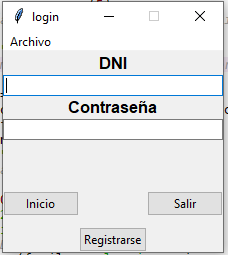
\includegraphics[scale=1]{Inicio} 
\caption{Pantalla de inicio del programa (Versión 2.0)}
\end{figure}
\subsubsection{Crear un Usuario/Registrarse}
Una vez abierto el programa, haga clic en el botón de \textbf{“Registrarse”}. 
\begin{figure}[htb]
\centering
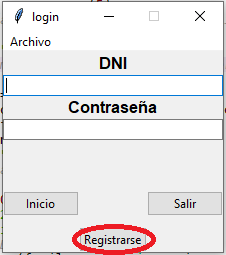
\includegraphics[scale=1]{inicioregistro} 
\caption{Pantalla de inicio, botón Registrar (Versión 1.0)}
\end{figure}

\begin{itemize}
\item	\textbf{DNI:} escriba su número del documento de DNI sin la letra, el cual será su usuario para iniciar sesión posteriormente. Ej: 71257992
\item	\textbf{Nombre:} escriba su nombre solo con letras, sin símbolos o signos.
\item	\textbf{Apellido:} escriba su nombre solo con letras, sin símbolos o signos.
\item	\textbf{Contraseña:} escriba la contraseña que quiere para iniciar sesión en la aplicación, sin límite de caracteres y/o símbolos.
\item	\textbf{Sexo:} marque su sexo haciendo clic encima del correspondiente.
\item	\textbf{Edad:} escriba su edad en números, sin letras o símbolos.
\item	\textbf{Altura:} escriba su altura en centímetros en números, sin letras o símbolos.
\item	\textbf{Peso:} escriba su peso en kilogramos en números, pudiendo incluir comas y decimales, pero no letras. Ej: 65,8
\item	\textbf{Actividad:} marque haciendo clic encima del número correspondiente al nivel de actividad que suele realizar. El significado de cada uno es:
\begin{itemize}
\item	1 - poco o ningún ejercicio.
\item	2 - ejercicio ligero (de 1 a 3 días por semana).
\item	3 - ejercicio moderado (de 3 a 5 días por semana).
\item	4 - ejercicio fuerte (6 días por semana).
\item	5 - ejercicio profesional o extremo.
\end{itemize}
\item	\textbf{Patología:} haga clic en el desplegable y seleccione si sufre alguna de las patologías sugeridas o “sin patología” en el caso de que no sea así.
\item	\textbf{Tipo:} marque haciendo clic encima del tipo de dieta que quiere, siendo:
\begin{itemize}
\item	Bajar - una dieta para bajar de peso de forma saludable.
\item	Mantener - una dieta para mantener el peso de forma saludable.
\item	Subir - una dieta para subir de peso de forma saludable.
\end{itemize}
\end{itemize}

Cuando haya rellenado todos los datos, pulse en el botón de “Aceptar y Guardar” para crear el usuario y guardar todos los datos que ha registrado (si falta algún campo por completar el programa dará error y no le permitirá guardar los cambios).
Se abrirá la siguiente ventana con los datos que deberá rellenar:
\imagen{registroguardar}{Ventana de registro del nuevo usuario señalizada para el registro (Version 1.0)}
También puede pulsar el botón de “Cancelar” si quiere salir cancelar el registro, o la “X” de la esquina de arriba a la derecha si desea cerrar la ventana.
\imagen{registrocerrar}{Ventana de registro del nuevo usuario señalizada para el cierre (Version 1.0)}
\subsubsection{INICIAR SESIÓN}
\imagen{LoginDetallado}{Inicio de sesión detallado (Versión 2.0)}
Para iniciar sesión en el programa con su usuario, escriba su DNI sin letra en el apartado llamado “DNI” (el cual será su número de usuario) y la contraseña que ha elegido anteriormente en la casilla denominada “Contraseña”. Cuando ya estén los dos campos rellenos con sus datos de usuario, pulse el botón de \textbf{''Inicio''} para iniciar el programa. Además, podrá encontrar el Manual de Usuario del programa en todo momento en la pestaña \textbf{``Archivo''}\\
Sino ha creado aún su usuario, acuda al apartado anterior del manual para seguir las instrucciones y registrarse.\\
Si desea salir o cerrar el programa, pulse el botón de “Salir” o la “X” de la esquina de arriba a la derecha.
\begin{figure}[htb]
\centering
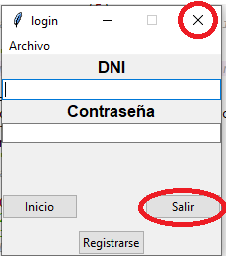
\includegraphics[scale=1]{InicioSalir} 
\caption{Imagen detallando el cierre del programa (Version 2.0}
\end{figure}

\subsection{PÁGINA PRINCIPAL}
\imagen{PagPrincipal}{Página principal de la aplicación (Version 1.0)}
\subsubsection{ARCHIVO}
\imagen{PPArchivo}{Pantalla Principal señalizando la opción Archivo (Versión 1.0)}
Arriba a la izquierda de la página encontrará el botón “Archivo”, en el que si pulsa se desplegarán otras tres opciones, las cuales se abrirán o ejecutarán haciendo clic sobre ellas.
\begin{itemize}
\item	\textbf{Manual:} contiene el manual de usuario, documento en el que encontrará las instrucciones de cómo utilizar el programa.
\item	\textbf{Guardar:} sirve para guardar la información o los cambios nuevos que haya realizado en el programa o su dieta personal. Recuerde pulsarlo si no quiere perder su progreso o los cambios realizados antes de cerrar el programa.
\item	\textbf{Salir:} sirve para salir y cerrar completamente el programa.
\end{itemize}
\subsubsection{ESTILOS}
\imagen{PPEstilos}{Pantalla Principal señalizando la opción estilos (Versión 1.0)}
En el apartado estilos encontrará un desplegable con las opciones de diseño que tiene el programa, con diferentes combinaciones de colores. Puede elegir el estilo que quiere clicando sobre su favorito.\\
El estilo se cambia cuando reinicie el programa. Una ventana que aparecerá después de seleccionarlo le informará de ello, pudiendo cerrarla del botón de “Aceptar” o la “X”.
\subsection{INFORMACIÓN DE USUARIO}
\imagen{InfUsuario}{Botón para pasar e la ventana de la información del usuario (Versión 1.0)}

En esta sección podrá consultar y modificar la información personal de su usuario. Si desea modificar sus datos debe pulsar en “Editar Información”, y se abrirá una nueva ventana en la que podrá cambiarlos. Los pasos a seguir son los mismos que durante el procedimiento de registro, ante cualquier duda acuda al punto 1.1. de este manual.\\
\imagen{editUsuario}{Botón para editar la información (Versión 1.0)}
\imagen{editInf}{Pantalla para editar la información del Usuario(Versión 1.0)}
Si desea volver a atrás o desechar los cambios realizados para que no se guarden, Haga Click en la opción de \textbf{“Cancelar”}. Y si una vez en su información de usuario quiere volver a la página principal, pulse \textbf{“Volver al Inicio”}.
\subsection{DIETA DIARIA}
\imagen{DietaDiaria}{Botón para pasar a la dieta diaria(Versión 1.0)}
\subsubsection{COMIDAS DEL DÍA}
Una vez haya entrado en la parte de \textbf{“Dieta Diaria”}, la ventana cambiará. Arriba aparecerán cinco pestañas con el nombre de cada una de las comidas del día (“Desayuno”, “Almuerzo”, “Comida”, “Merienda” y “Cena”) que podrá abrir pulsando en ellas.\\
\imagen{cincocomidas}{Pantalla principal de mostrar dieta(Versión 1.0)}

Cuando abra cualquiera de las comidas, aparecerán tres posibles opciones de menú, las más saludables para ese momento del día. Si pulsa en ellas, a su derecha se mostrará la descripción de cada plato con sus kilocalorías (“Kcal”), los hidratos de carbono (“Hidratos”), las proteínas, las grasas y la calidad. La calidad se representará con las letras A-B-C-D-E siendo A la opción más saludable y E la peor.\\

Una vez seleccionado el plato que desea, clique en \textbf{“Seleccionar”} para confirmar su elección.\\

En la parte baja de la pantalla, se irán registrando las cinco comidas que haya ido seleccionando cada día para poder visualizarlas rápidamente.\\
\imagen{infoPlato}{Información del plato y selecciones del día (Version 1.0)}
Si el plato que ha seleccionado finalmente no es el que desea, debe pulsar el botón de \textbf{“Editar”}. De esta forma, se desmarcará la opción elegida anteriormente y el programa le permitirá elegir de nuevo.\\
\imagen{editPlato}{Selección de comida y guardado de la elección (Version 1.0)}
Si desea volver a la página principal, pulse \textbf{“Volver al Inicio”}.
\subsubsection{REFRESCAR}
La opción de \textbf{“Refrescar”} nos permite cambiar las tres opciones de comida sugeridas, por si no fuese de su agrado o no le apeteciese en concreto ninguna de las sugerencias. Pulsando en el botón, aparecerán otras tres diferentes, pudiendo actualizarlas las veces que el usuario desee.\\

Se debe tener en cuenta que cada vez que se refresque, las nuevas alternativas sugeridas empeorarán en calidad progresivamente, dificultando su objetivo de comer adecuadamente.\\

En la esquina derecha inferior de la ventana aparece una \textbf{barra de progreso}, indicando la calidad de los platos que ha elegido, y por lo tanto lo saludable que ha sido o está siendo su alimentación del día (varía con cada selección). La calidad de sus elecciones estará representada con los colores del semáforo verde-amarillo-naranja-rojo, verde la opción mas adecuada y rojo la peor. Esto le permitirá aprender las comidas que son más saludables y rectificar si desea mejorar en alguna de ellas.\\
\imagen{refrescar}{Resultados del botón refrescar (Versión 1.0)}
\imagen{nutriscoreMasMenosSal}{Caliad Nutriscore}
\subsubsection{AÑADIR PLATO}
\imagen{AddAlimento}{Botón añadir alimento (Versión 1.0)}
\imagen{addAlimento2}{Formulario para añadir un nuevo alimento (Versión 2.0)}
Si el usuario desea añadir un plato nuevo, debe pulsar en \textbf{“Añadir Alimento”} abajo a la izquierda de la ventana. Así, aparece una nueva ventana con hasta cuatro columnas para añadir en cada una de ellas los ingredientes que compongan cada comida. Deberá ir rellenando sus componentes por cada 100 gramos de alimento.
\begin{itemize}
\item	\textbf{Nombre:} solo letras, sin números o símbolos.
\item	\textbf{Gramos:} solo valores numéricos, sin letras o símbolos.
\item	\textbf{Kilocalorías:} solo valores numéricos, sin letras o símbolos.
\item	\textbf{Grasas:} solo valores numéricos, sin letras o símbolos.
\item	\textbf{Grasas saturadas (“Saturadas”):} solo valores numéricos, sin letras o símbolos.
\item	\textbf{Hidratos de carbono (“Hidratos”):} solo valores numéricos, sin letras o símbolos.
\item	\textbf{Fibra:} solo valores numéricos, sin letras o símbolos.
\item	\textbf{Azúcares:} solo valores numéricos, sin letras o símbolos.
\item	\textbf{Proteína:} solo valores numéricos, sin letras o símbolos.
\item	\textbf{Sodio:} solo valores numéricos, sin letras o símbolos.
\end{itemize}
\imagen{addAlimento3}{Partes del formulario (Versión 2.0)}
También deberá elegir el \textbf{tipo de comida} que es su plato (desayuno, almuerzo, comida, merienda y/o cena) pulsando sobre ellas, pudiéndose marcar varias opciones si fuese necesario.\\
\imagen{selecTipo}{Opciones del tipo comida (V.1.0)}
Cuando todos los campos mencionados hayan sido completados, pulse \textbf{“Validar”} para aceptar o confirmar el plato, o “Cancelar” si desea volver a atrás o desechar los cambios realizados para que no se guarden.\\
\imagen{validar3}{Pantalla de validación de alimento (Versión 1.2)}

Al validar el plato, el programa lo crea y muestra un gráfico, el cual tiene en el eje X u Horizontal la calidad de los alimentos y en el eje Y o Vertical, el número de alimentos que tienen esa calidad, por si el usuario desease modificar el plato o alguno de sus ingredientes. Para terminar haga clic en \textbf{“Guardar”} y el plato quedará registrado definitivamente, o \textbf{“Cancelar”} para editarlo o salir porque no desea guardarlo.\\

Si desea volver a la página de dietas diarias, pulse \textbf{“Cancelar”}.

\subsection{HISTORIAL}

\imagen{historial2}{Botón Historial(Versión 1.0)}
En los gráficos que aparecen en este apartado se muestra una línea que representa la calidad de las elecciones que se han realizado en cada comida, clasificándolo de menos saludable (puntos más altos en la representación) a lo más saludable (puntos más bajos en la representación).
Los diferentes gráficos que podrá visualizar pulsando en cada uno de ellos serán:
\begin{itemize}
\item	Gráfico total mensual.
\item	Gráfico desayuno.
\item	Gráfico almuerzo.
\item	Gráfico comida.
\item	Gráfico merienda.
\item	Gráfico cena.
\item	Semana ingerida.
\end{itemize}	

Si desea volver a la página principal, pulse “Volver al Inicio”.
\imagen{graficos}{Pantalla del Historial (V.1.0)}
\subsubsection{GRÁFICOS}
Existen dos tipos de gráficos:
\begin{enumerate}
\item \textbf{Gráfico total:} gráfico que muestra la media de la calidad que el usuario toma en un día completo, con todos los alimentos. El eje horizontal o X representa los días, y el eje vertical o Y es la media de la calidad.
\item \textbf{Gráfico de desayuno, almuerzo, comida, merienda o cena:} tienen la misma función que el gráfico total, pero de cada comida específica, así podrá observar en cuales come peor o mejor.
\end{enumerate}
\subsubsection{SEMANA INGERIDA}
\imagen{SemIng2}{Pantalla de muestra de la semana ingerida (Versión 1.0)}
Cuando se escoge la opción de la semana ingerida, se muestra una lista de lo que el usuario ha comido en los últimos siete días. Sino se escogió nada para esa comida aparece “NaN”.
\section{Guía de errores, avisos e informes}
A lo largo del uso de la aplicación se pueden encontrar con diferentes ventanas emergentes que informan del estado de la aplicación. Estas ventanas informarán de la situación del programa y del motivo por el que surgen dichas ventanas.
Nos podemos encontrar tres tipos de ventanas:
\begin{enumerate}
\item \textbf{Información} - Ventanas que informan de que se ha guardado correctamente. En la mayoría de ocasiones, se deberá reiniciar el programa para ver los cambios.
\imagen{Informacion}{Ventana emergente de información}
\item \textbf{Avisos} - Ventana que informa de que no se ha podido llevar a cabo la acción realizada por un fallo menor. Indica cual es el fallo para que se pueda solucionar.
\imagen{Aviso}{Ventana emergente de avisos}
\item \textbf{Error} - Ventana que indica que ha sucedido un error grave, y que le programa a dejado de funcionar. Pruebe a eliminar y reinstalar el programa.
\imagen{Error}{Ventana de error}
\end{enumerate}


\bibliographystyle{plain}
\bibliography{bibliografiaAnexos}

\end{document}
